\subsection{Iteration \#1}
\vspace{-0.6cm}
I iteration 1 arbejdes der med blokke som dækker over systemets mest grundlæggende funktionalitet. Batteri, ESC’er, motorer og sensorer tilsluttes dronen, og dronen gøres desuden i stand til oprette forbindelse til webapplikationen via 3G-shield’et.
Server opsættes, så basal kommunikation mellem dronen og server er muligt, bla. skal det være muligt for dronen at uploade sin nuværende position til server. For flere detaljer vedrørende opsætning og funktionalitet af server henvises til data view'et. 

\subsubsection*{User story}
\vspace{-0.4cm}
Bruger tænder dronen ved at tilslutte batteri. Main controller samt 3G/GPS module initialiseres og nuværende GPS position opdateres. Herefter opretter dronen forbindelse til webapplikation og sender information om sin nuværende GPS position. Fra webapplikationen er det muligt for bruger løbende at observere hvorvidt dronen er online og på hvilken GPS position dronen sidst har befundet sig.

%kommentar
\begin{figure}[H]
	\centering
	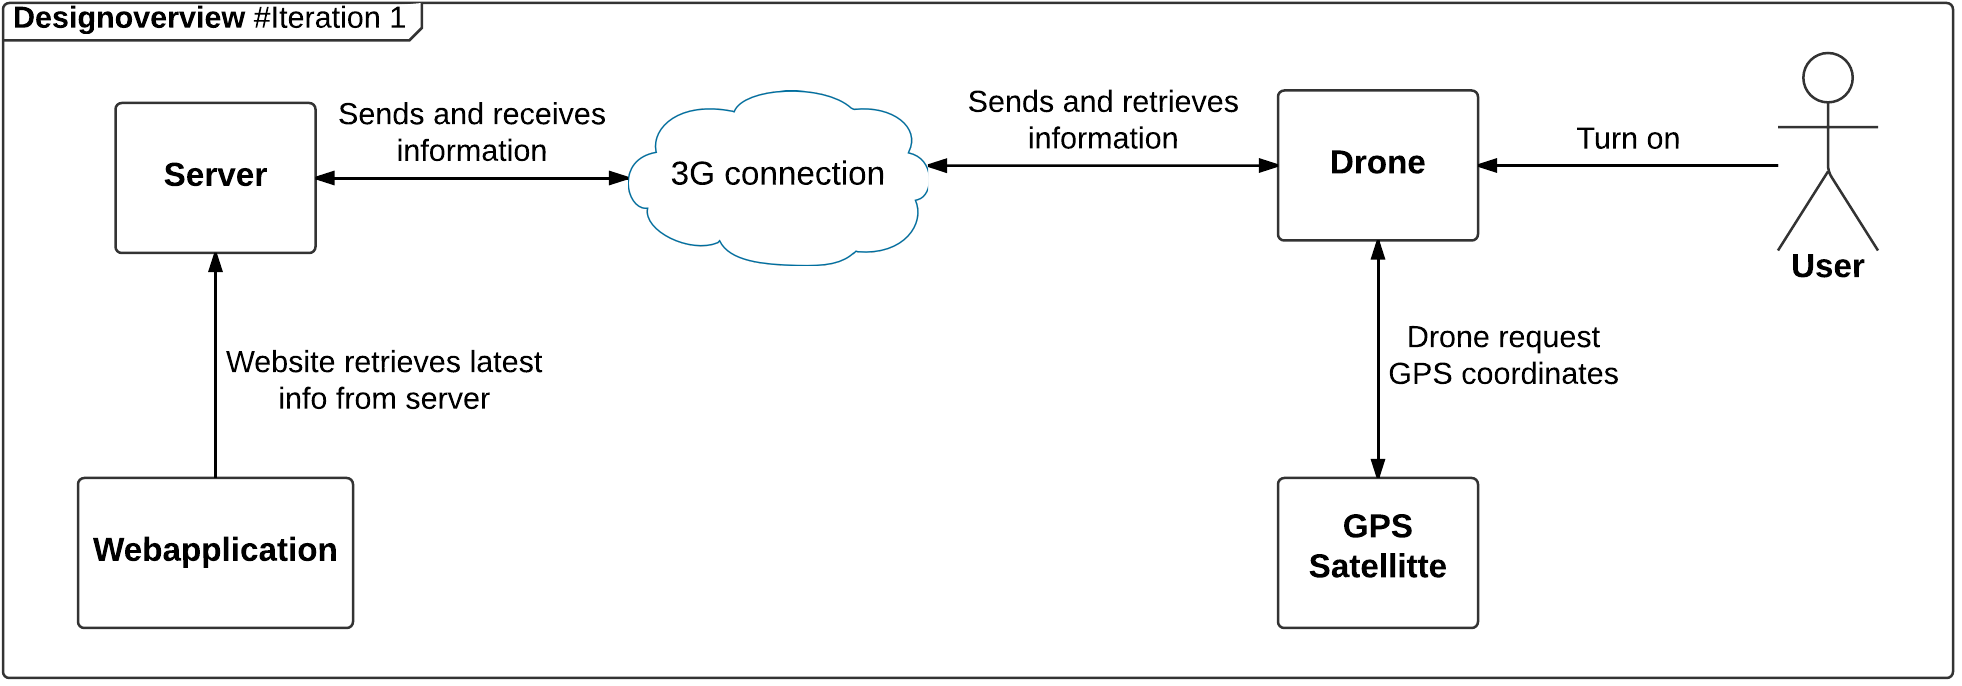
\includegraphics[width=1\textwidth]{Billeder/design_overview/design_overview_iteration1.png}
	\vspace{-.7cm}
	\caption{Designoverview}
	\label{fig:design_overview_iteration_1}
\end{figure}


\newpage
\subsubsection*{Pakkediagram drone}

I dette afsnit vises pakkediagram tilhørende drone. De pakker der vises i pakkediagrammet består af en eller flere klasser, der med stort samspil udfører opgaver indenfor et fælles ansvarsområde. På hver pakke findes en lille beskrivelse, der tydeliggør pakkens ansvarsområde. 


\begin{figure}[H]
	\centering
	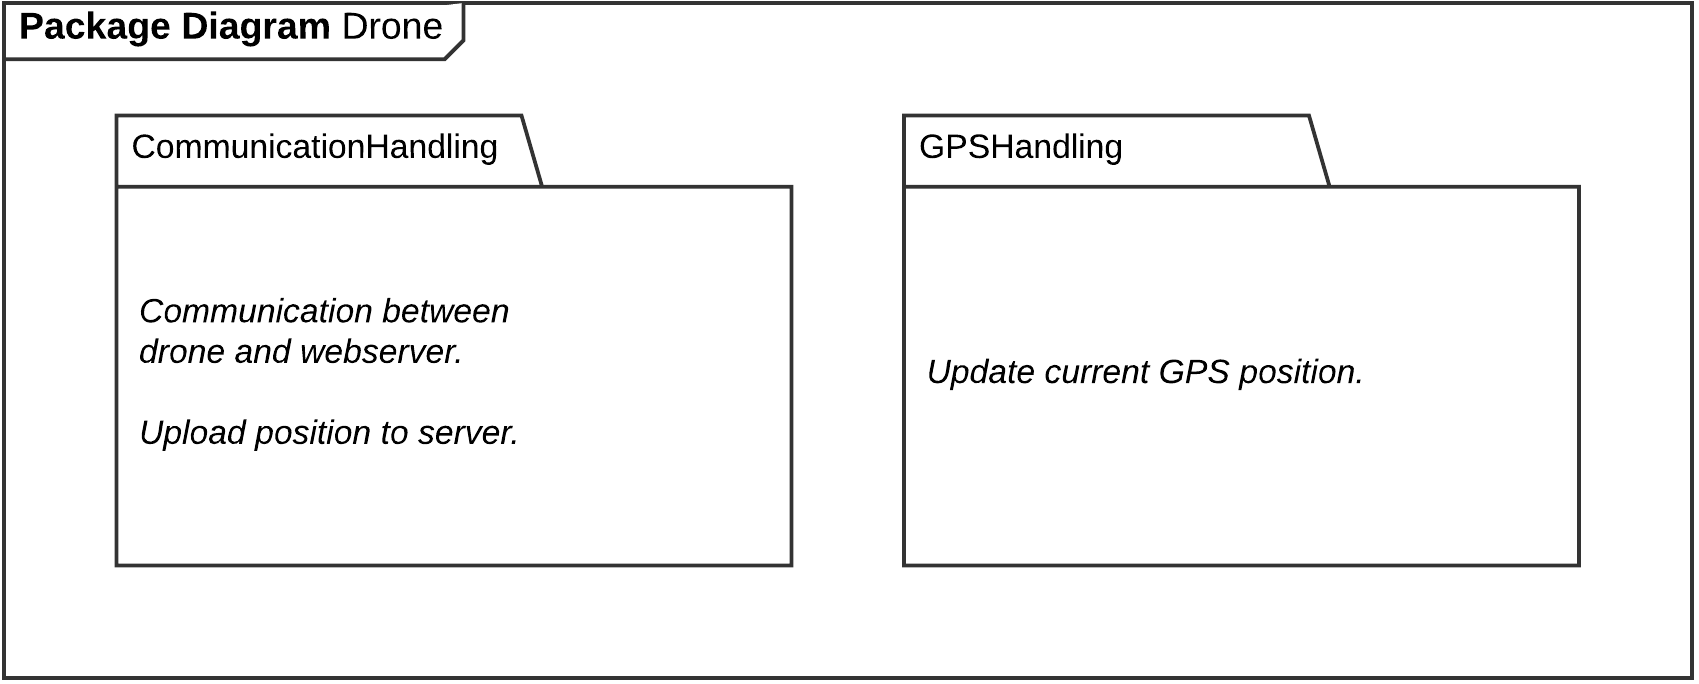
\includegraphics[width=1\textwidth]{Billeder/pakke_diagrammer/iteration1_drone.png}
	\vspace{-0.5cm}
	\caption{Pakkediagram drone}
	\label{fig:iteration1_pakke_diagram_drone}
\end{figure}

\textbf{CommunicationHandling}\\
Pakkens ansvar er kommunikation imellem drone og server. I denne iteration er der fokus på, at dronen skal kunne sende sin nuværende GPS position til server.

\textbf{GPSHandling}\\
Pakkens ansvar er håndtering af GPS. Dels er pakken ansvarlig for opstart og initiering af GPS, og desuden bruges pakken hver gang dronens nuværende GPS position skal opdateres.

\newpage
\subsubsection*{Pakkediagram webapplikation}

I dette afsnit vises pakkediagram tilhørende webapplikationen. De pakker der vises i pakkediagrammet består af en eller flere klasser, der med stort samspil udfører opgaver indenfor et fælles ansvarsområde. På hver pakke findes en lille beskrivelse, der tydeliggør pakkens ansvarsområde. 

\begin{figure}[H]
	\centering
	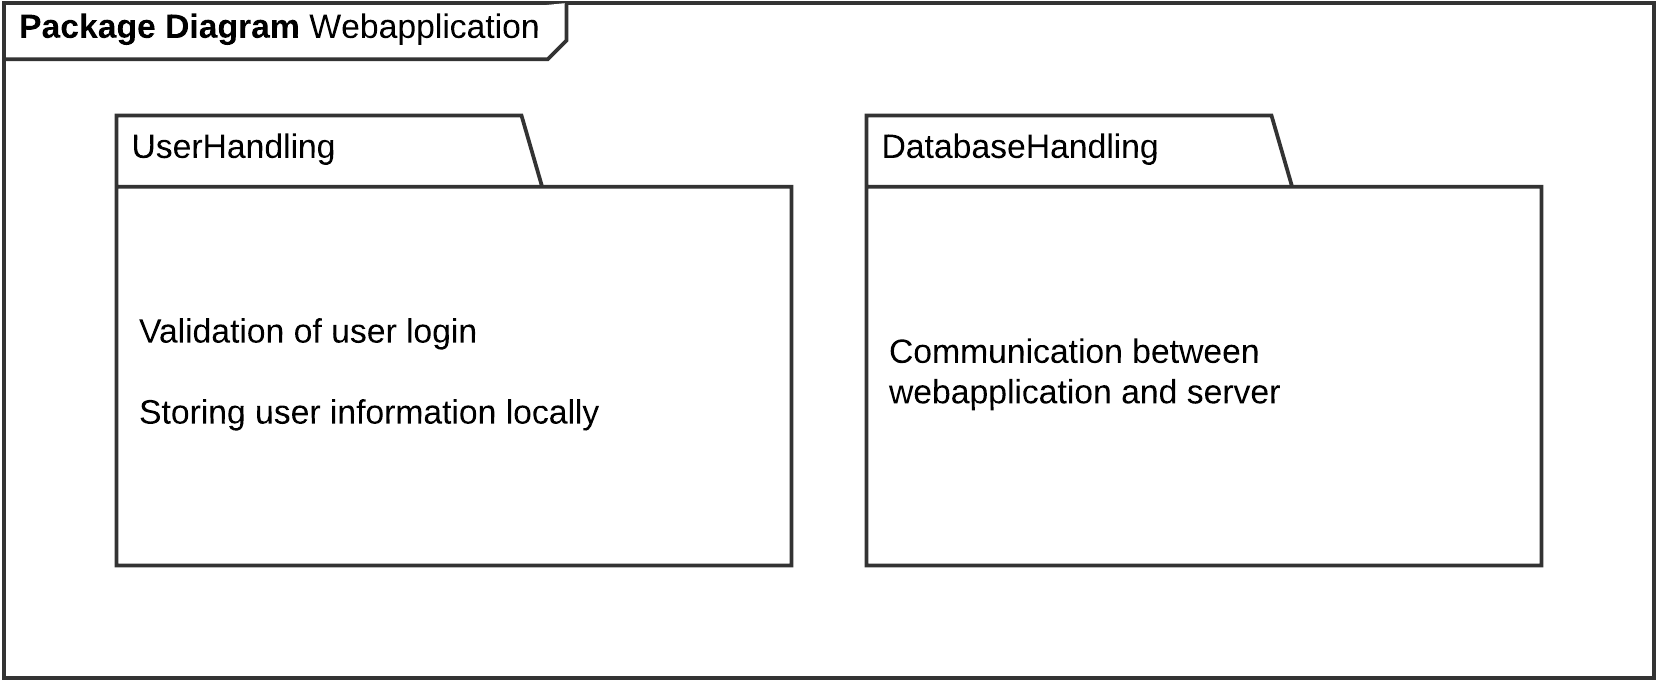
\includegraphics[width=1\textwidth]{Billeder/pakke_diagrammer/iteration1_server.png}
	\vspace{-0.5cm}
	\caption{Pakkediagram webapplikationen}
	\label{fig:iteration1_pakke_diagram_webapp}
\end{figure}

\textbf{UserHandling}\\
Pakkens ansvar er validering af login/log ud på webapplikationen. Pakken har også ansvaret for at hente og gemme data om den pågældende bruger.

\textbf{DatabaseHandling}\\
Pakkens ansvar er kommunikation imellem database og server. 


\newpage
\subsubsection*{Sekvensdiagram drone}
På sekvensdiagrammet på figur \ref{fig:Sekvens_diagram_iteration1}, vises hvilke klasser der indgår og bruges i første iteration. Af sekvensdiagrammet fremgår det, at sekvensen først startes når bruger tilslutter batteri og tænder dronen. Når der er tilkoblet forsyning initialiseres main controller samt 3G/GPS og nuværende GPS position  (longitude og latitude) opdateres. Dronens nuværende GPS position sended via PUT requests til webapplikationen. PUT requests bruges dels til at fortælle webapplikationen at dronen er online og dels til at give webapplikationen information om dronens nuværende position. 

%kommentar
\begin{figure}[H]
	\centering
	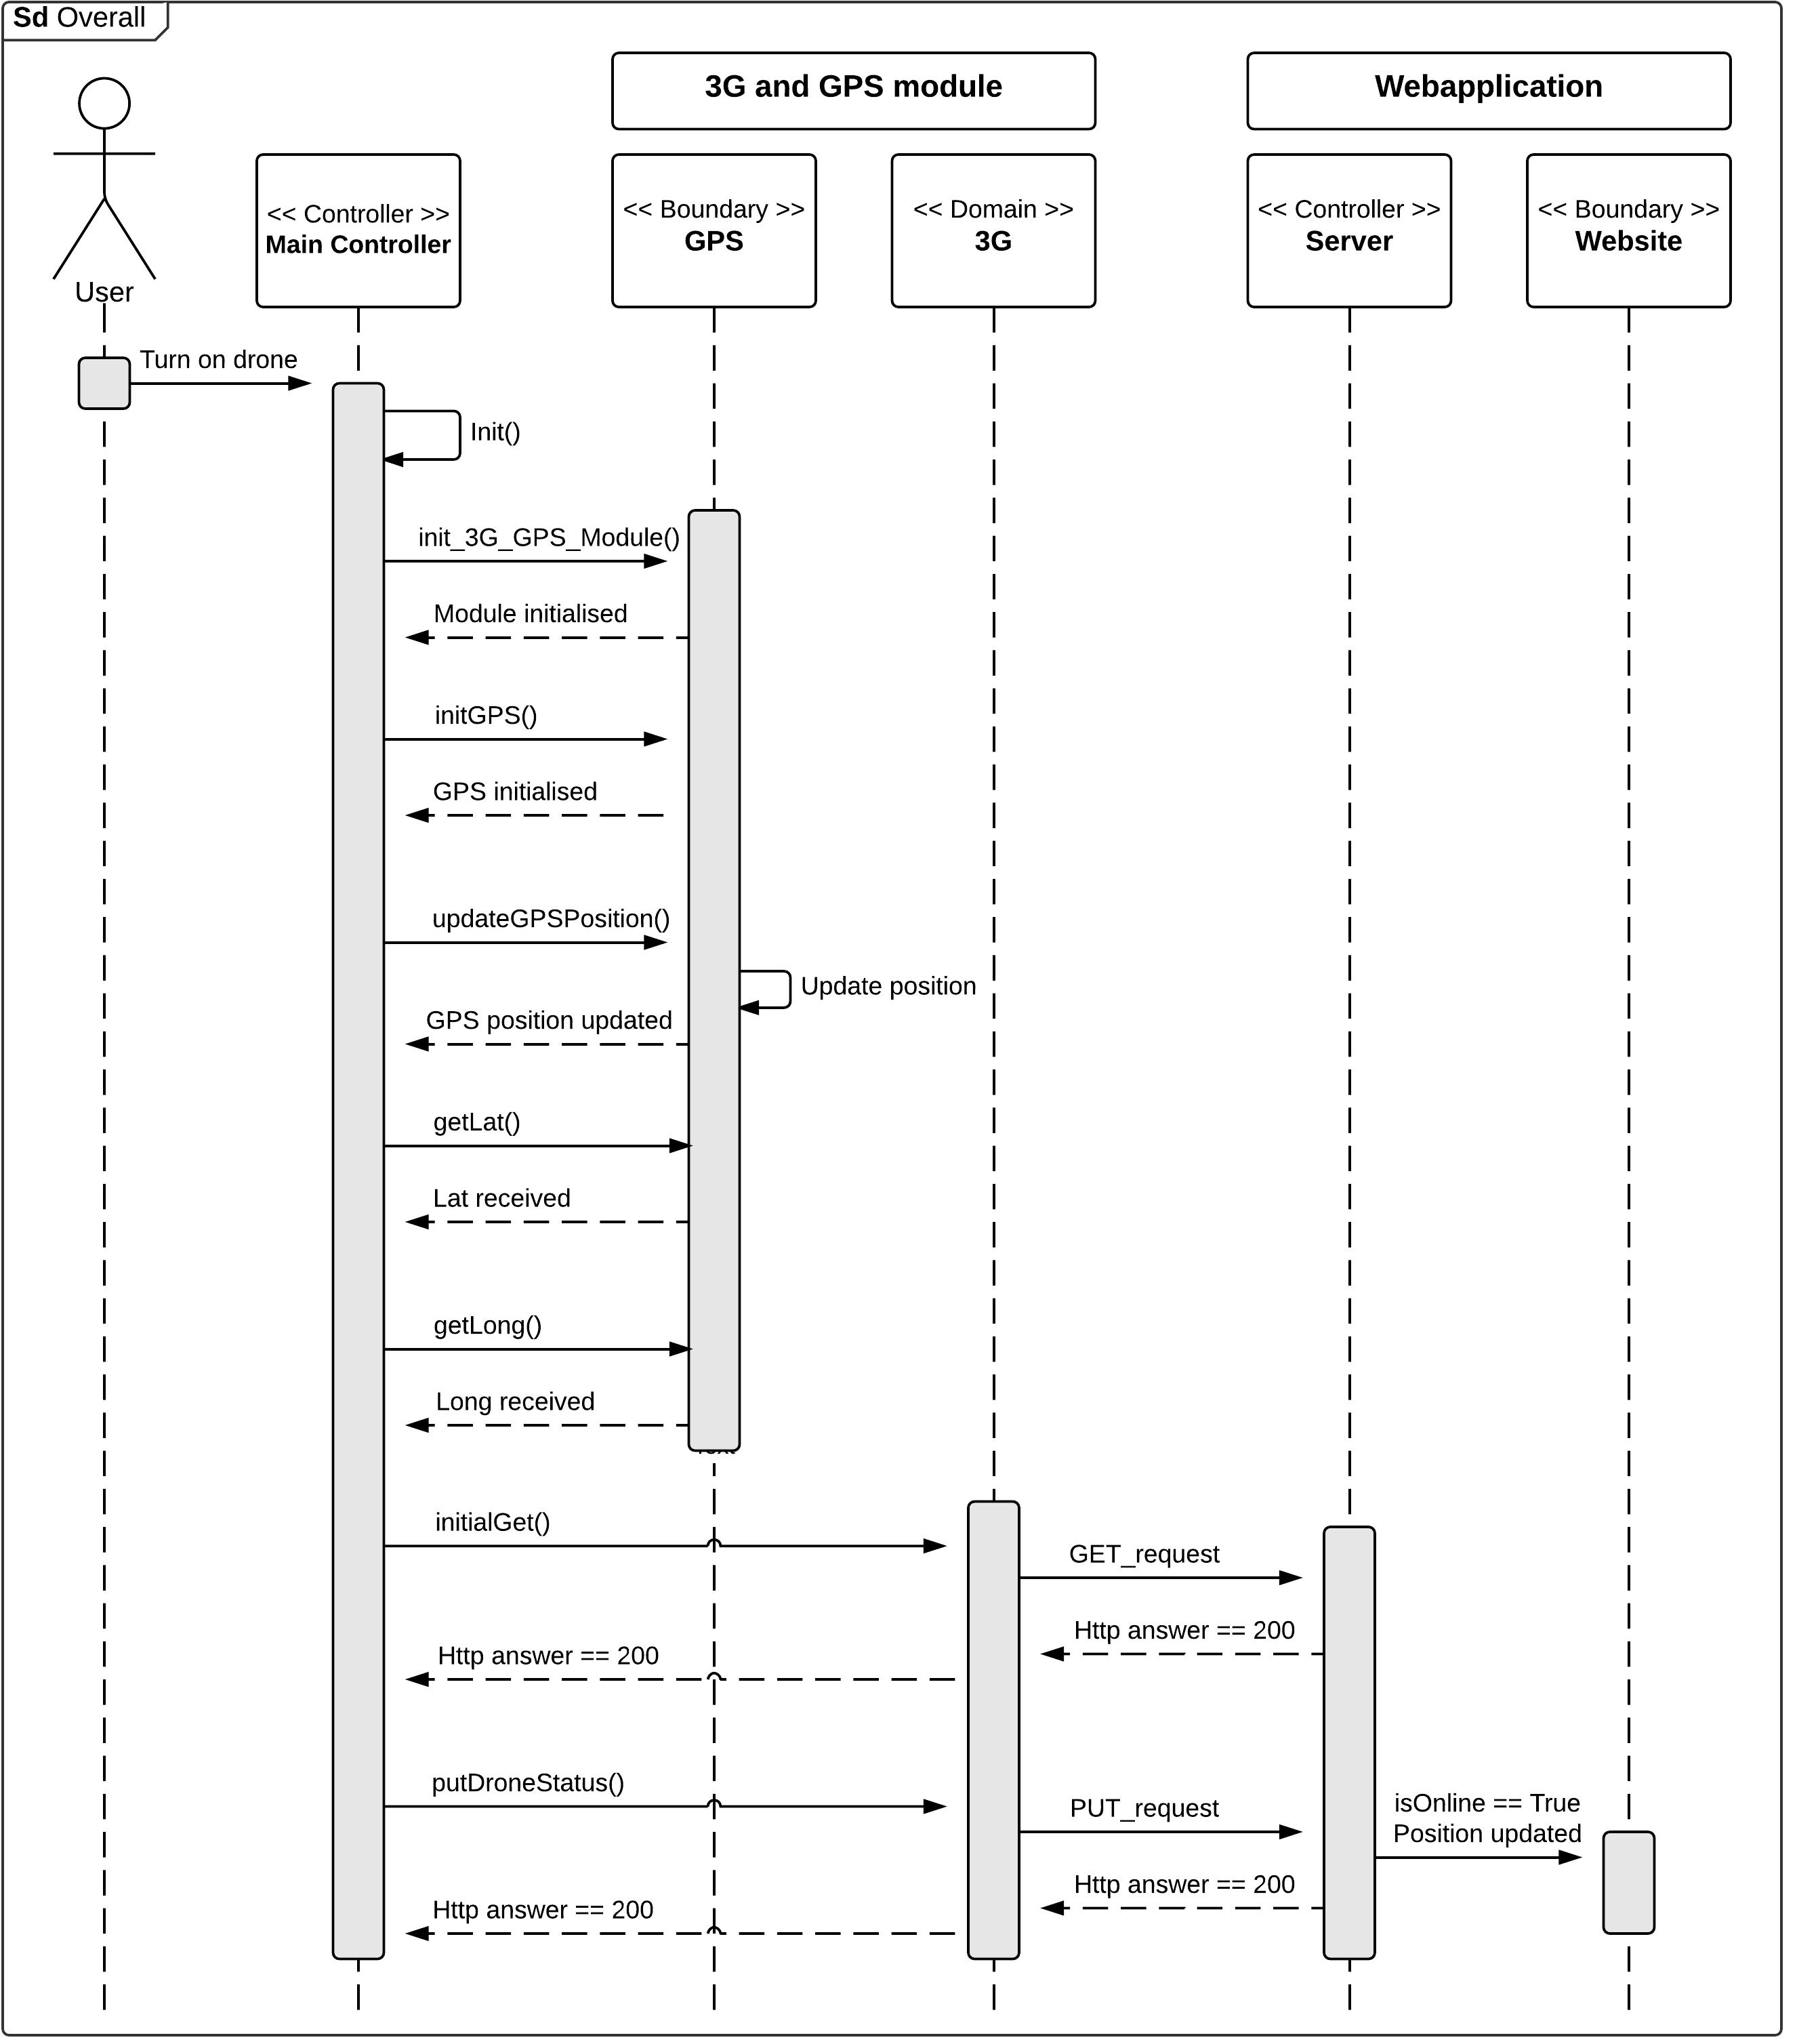
\includegraphics[width=1\textwidth]{Billeder/sekvens/sekvens_iteration1}
	\caption{Overordnet sekvensdiagram}
	\label{fig:Sekvens_diagram_iteration1}
\end{figure}
\newpage

Da boundary klassen \textit{3G} benytter tre underliggende klasser til håndtering af GET og PUT requests er sekvensdiagrammet på figur \ref{fig:Sekvens_diagram_iteration1} simplificeret. Sekvensdiagrammerne på figur \ref{fig:Sekvens_diagram_initialget} og \ref{fig:Sekvens_diagram_putDroneStatus} vises detaljeret hvordan 3G og underliggende klasser bruges til GET og PUT. \\

Sekvensdiagrammet på figur \ref{fig:Sekvens_diagram_initialget} viser hvilke klasser der anvendes til håndtering af GET. 

\begin{figure}[H]
	\centering
	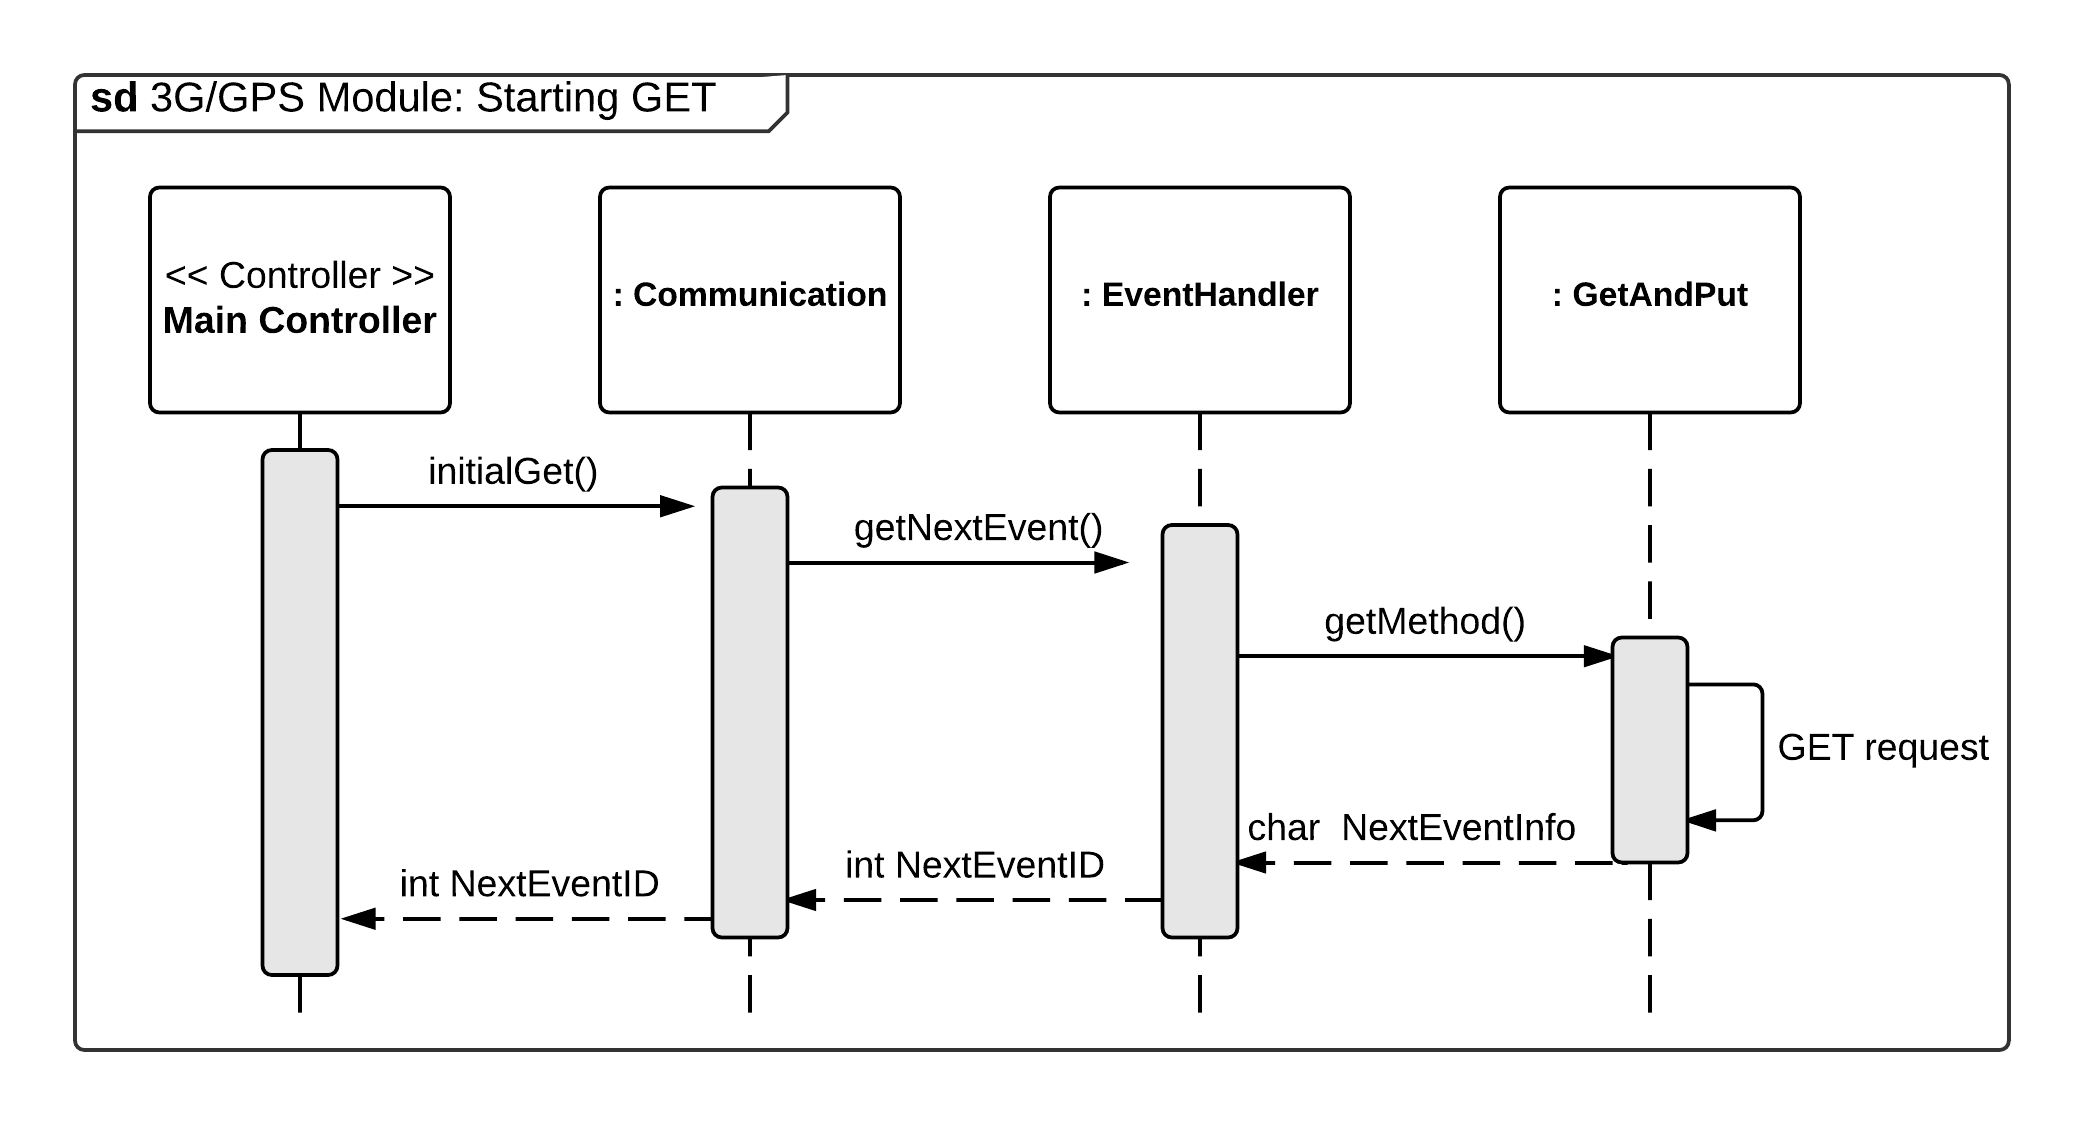
\includegraphics[width=1\textwidth]{Billeder/sekvens/sekvens_iteration1_initialget}
	\caption{Sekvensdiagram - initialget}
	\label{fig:Sekvens_diagram_initialget}
\end{figure}

\vspace{.5cm}

Sekvensdiagrammet på figur \ref{fig:Sekvens_diagram_putDroneStatus} viser hvilke klasser der anvendes til håndtering af PUT. 

\begin{figure}[H]
	\centering
	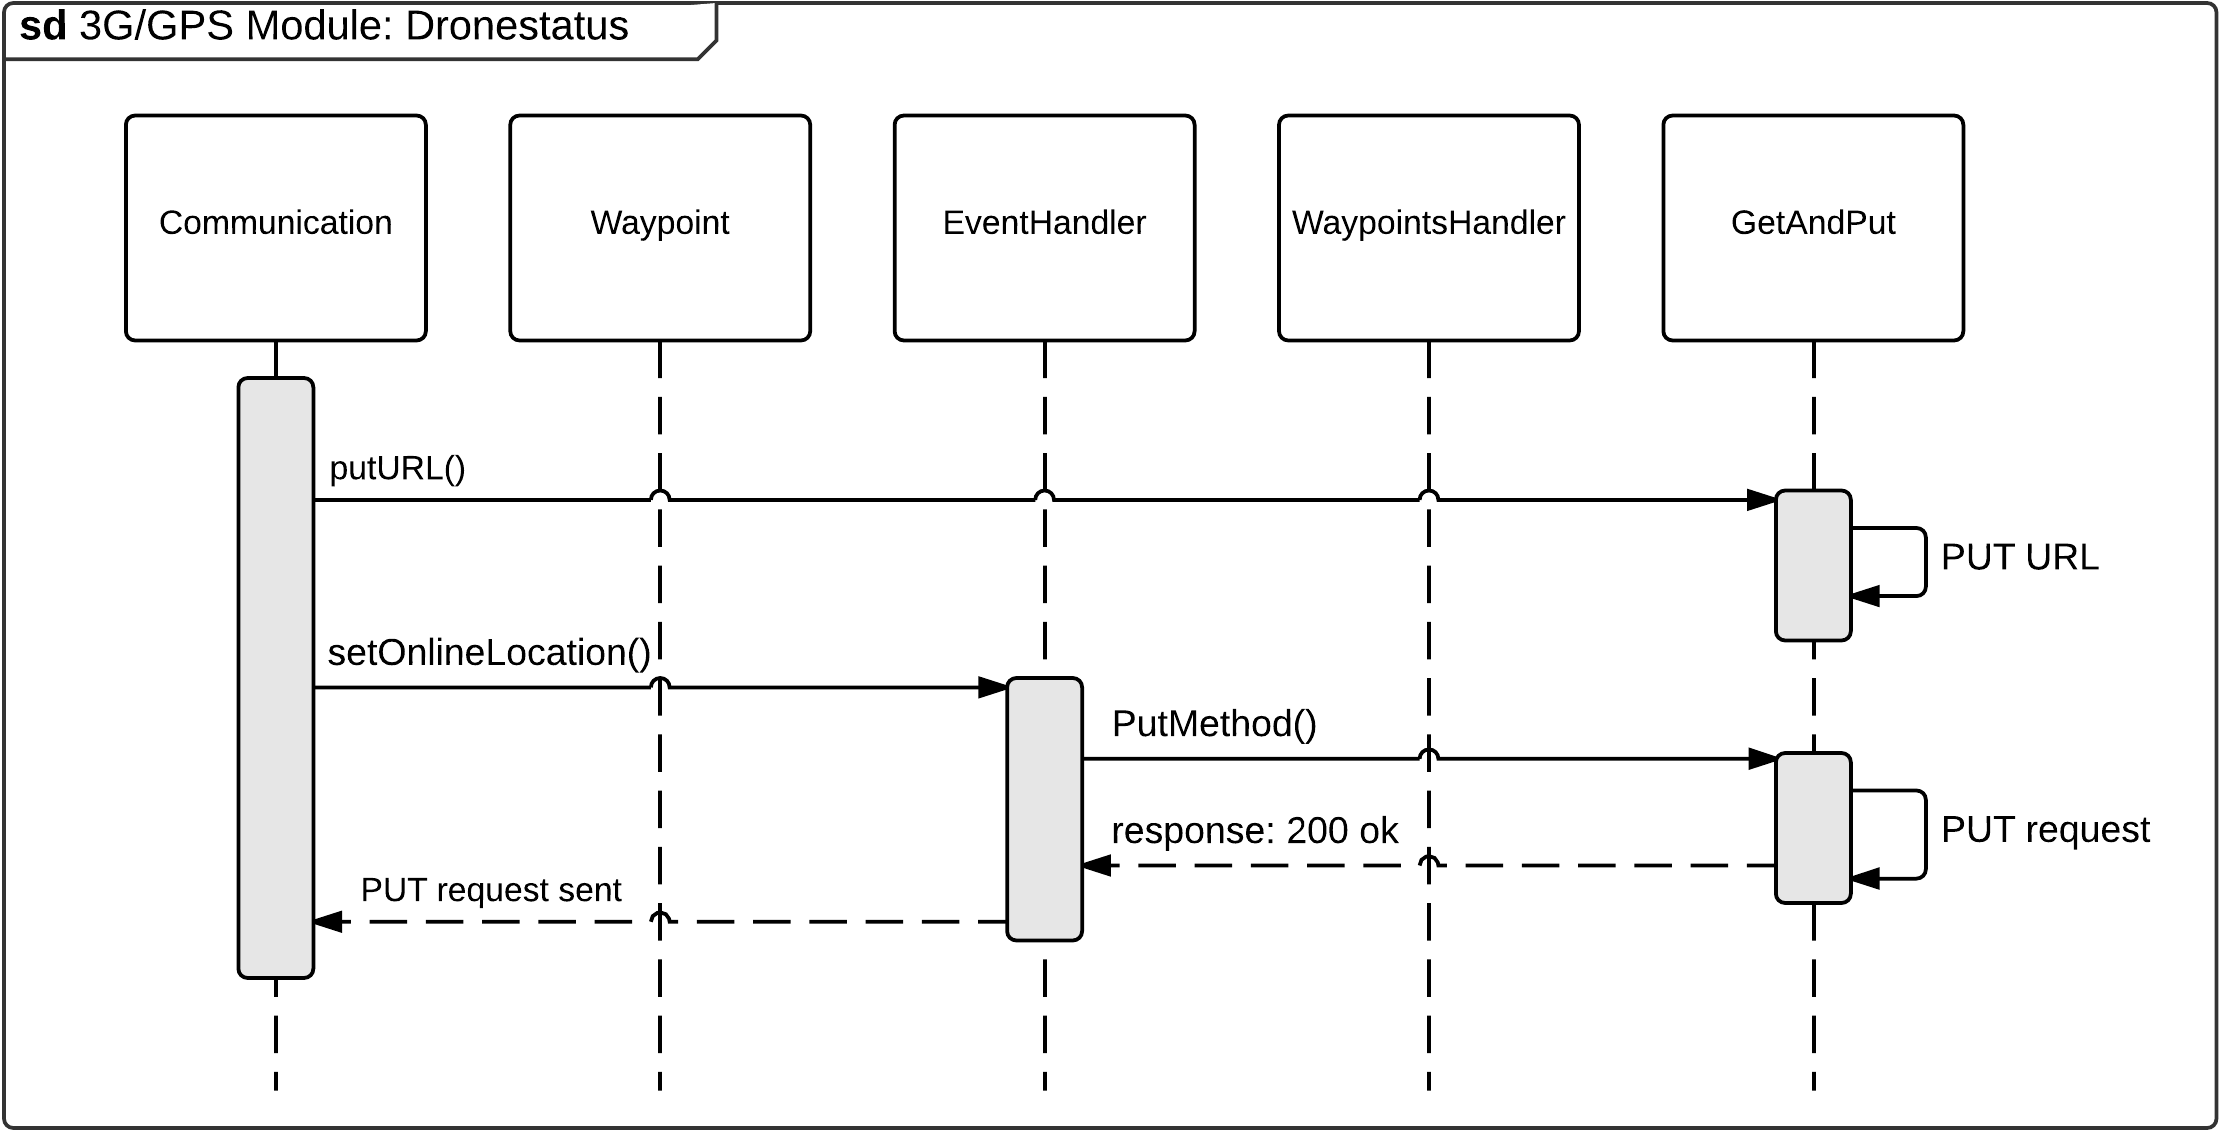
\includegraphics[width=1\textwidth]{Billeder/sekvens/sekvens_iteration1_putdronestatus}
	\caption{Sekvensdiagram - putDroneStatus}
	\label{fig:Sekvens_diagram_putDroneStatus}
\end{figure}


\newpage

\subsubsection*{Sekvensdiagram webapplikation}
På figur \ref{fig:Sekvens_diagram_login} ses sekvens diagrammet over login på webappplikationen. På diagrammet vises det at systemets bruger først bliver ført til næste side ved succesfuld login. Diagrammet viser også kommunikationen med CRUDServiceDrone som kommunikerer med databasen. Ydermere viser diagrammet hvordan AuthenticationServices håndterer bruger data.

\begin{figure}[H]
	\centering
	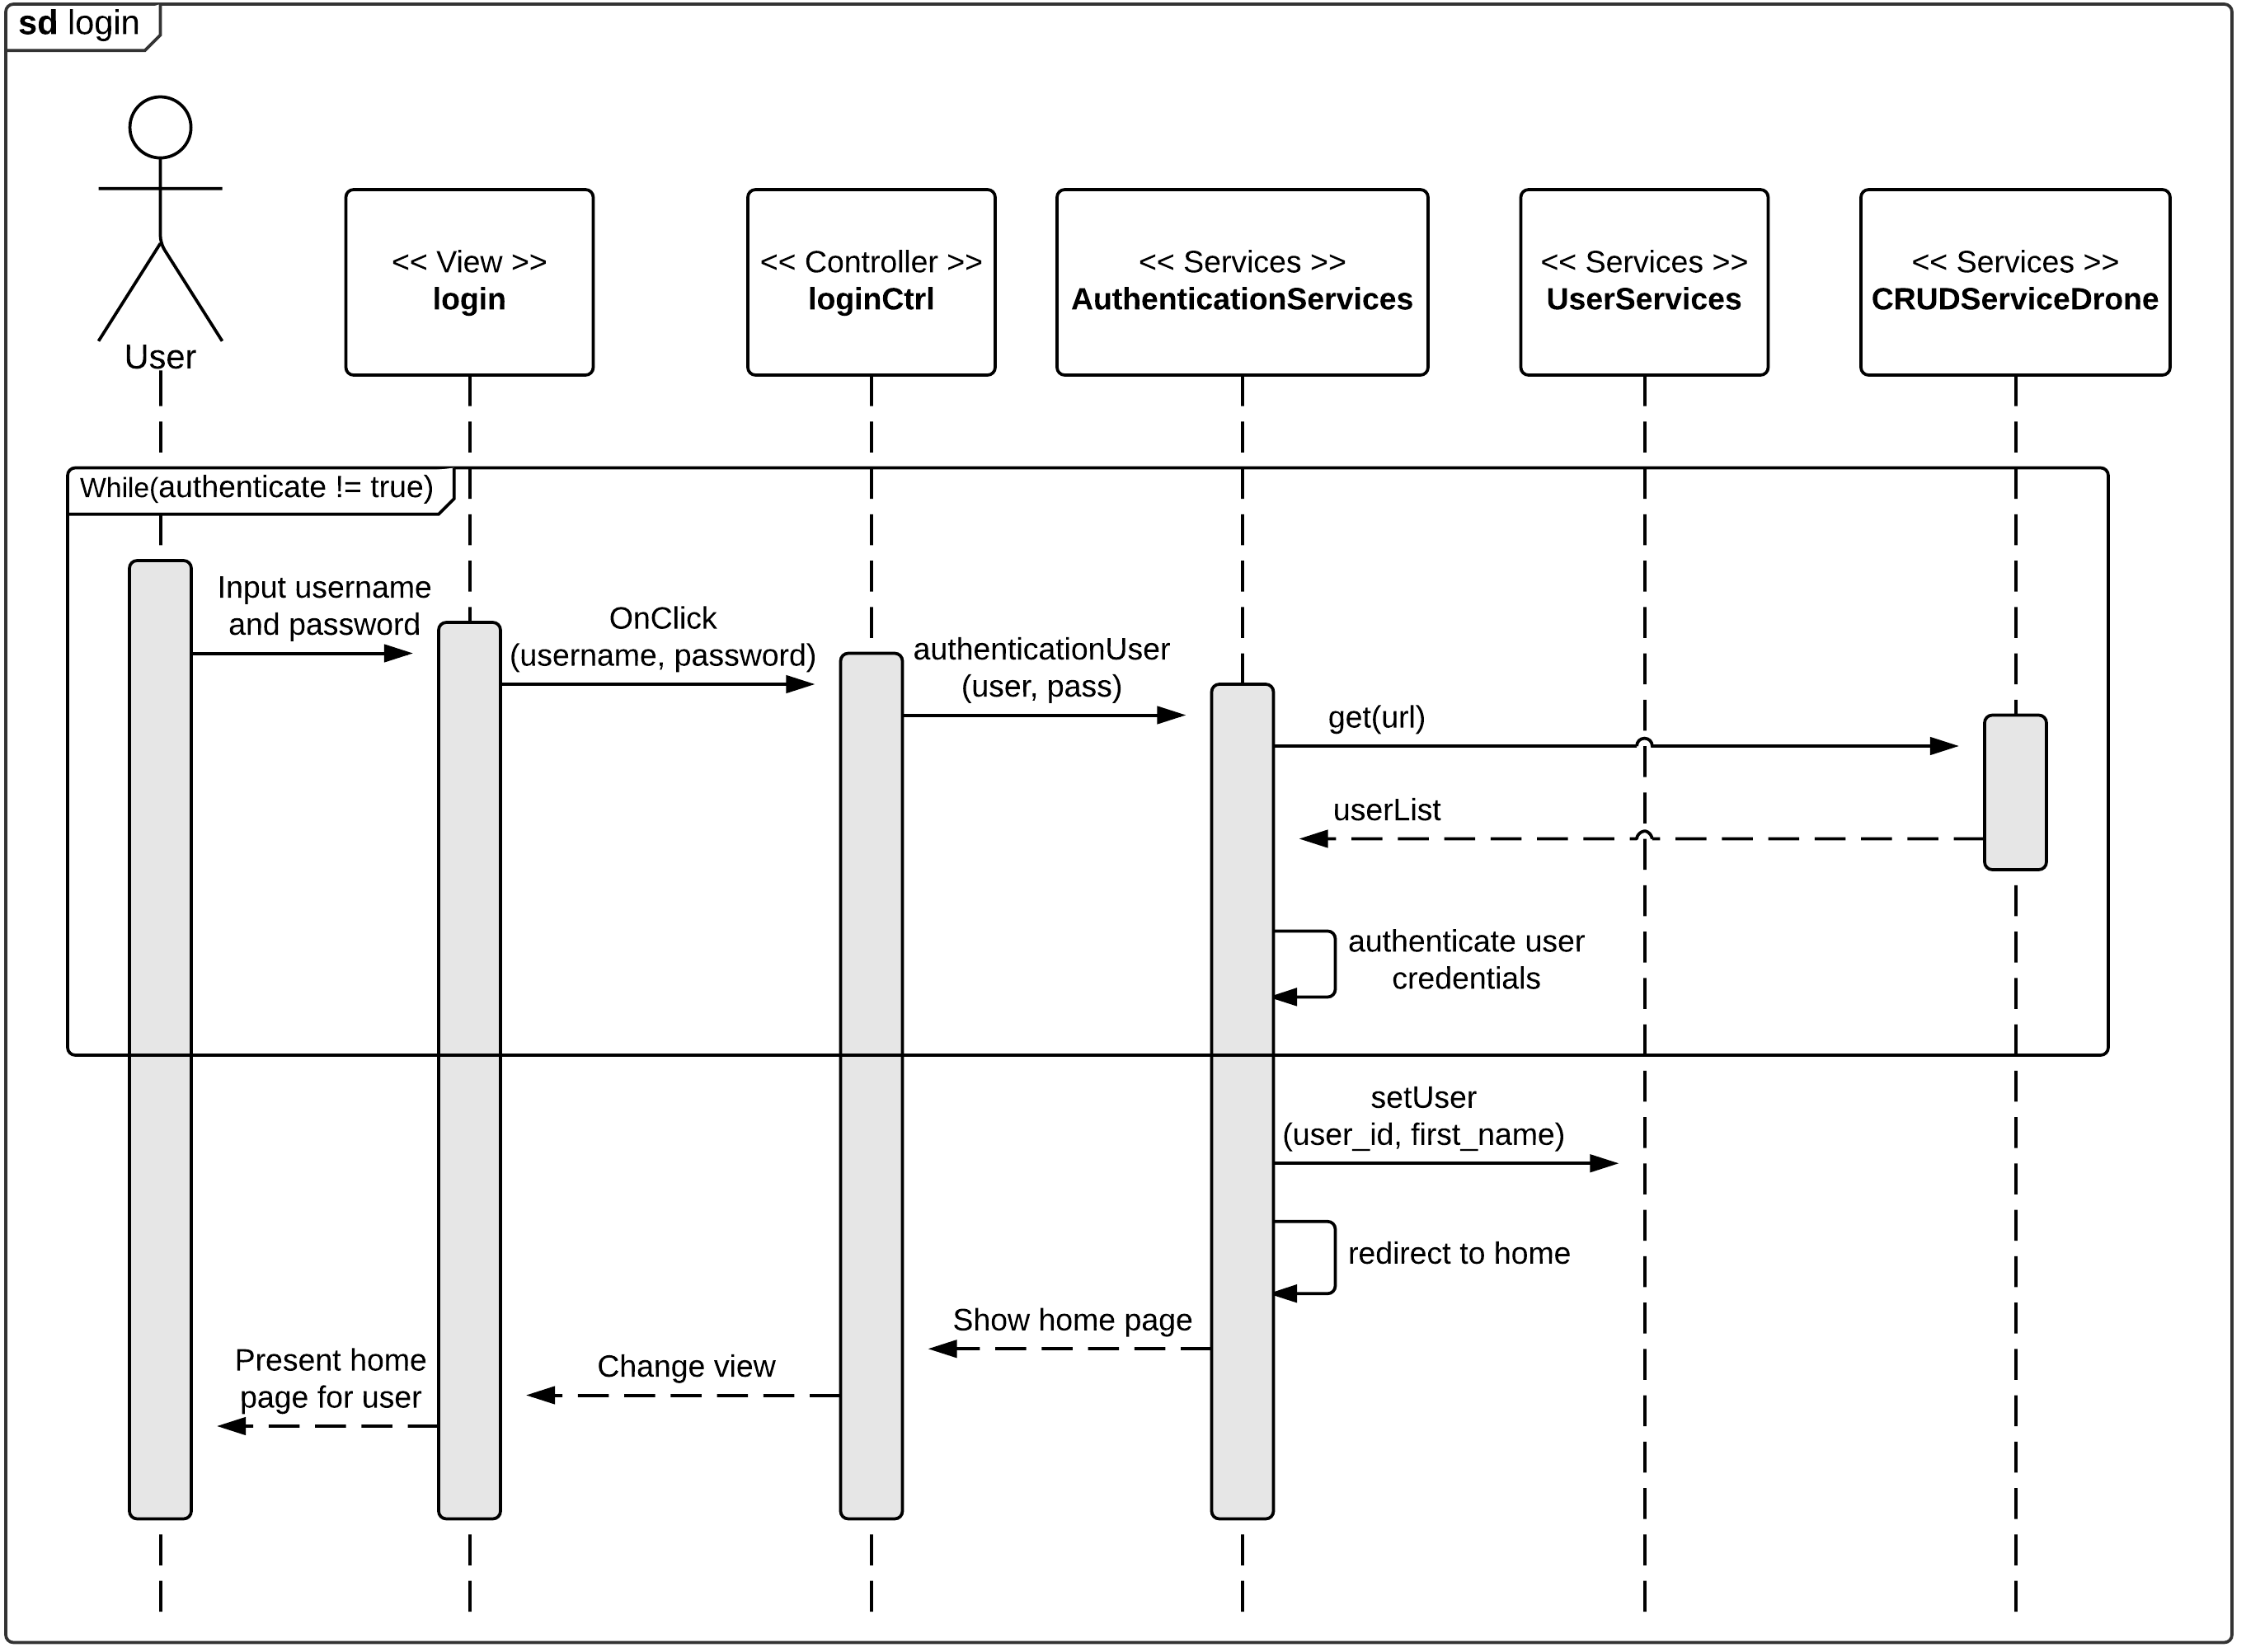
\includegraphics[width=1\textwidth]{Billeder/sekvens/login_sq_diagram.png}
	\caption{Sekvensdiagram - login}
	\label{fig:Sekvens_diagram_login}
\end{figure}
\newpage


\subsubsection*{Klassediagram drone}
\vspace{-0.2cm}
På figur \ref{fig:classDiagram_iteration1} vises et klassediagram som viser iterationens klasser, samt deres tilhørende metoder og attributter. På den følgende side forefindes en kort beskrivelse klasserne og deres ansvarsområder.

%kommentar
\begin{figure}[H]
	\centering
	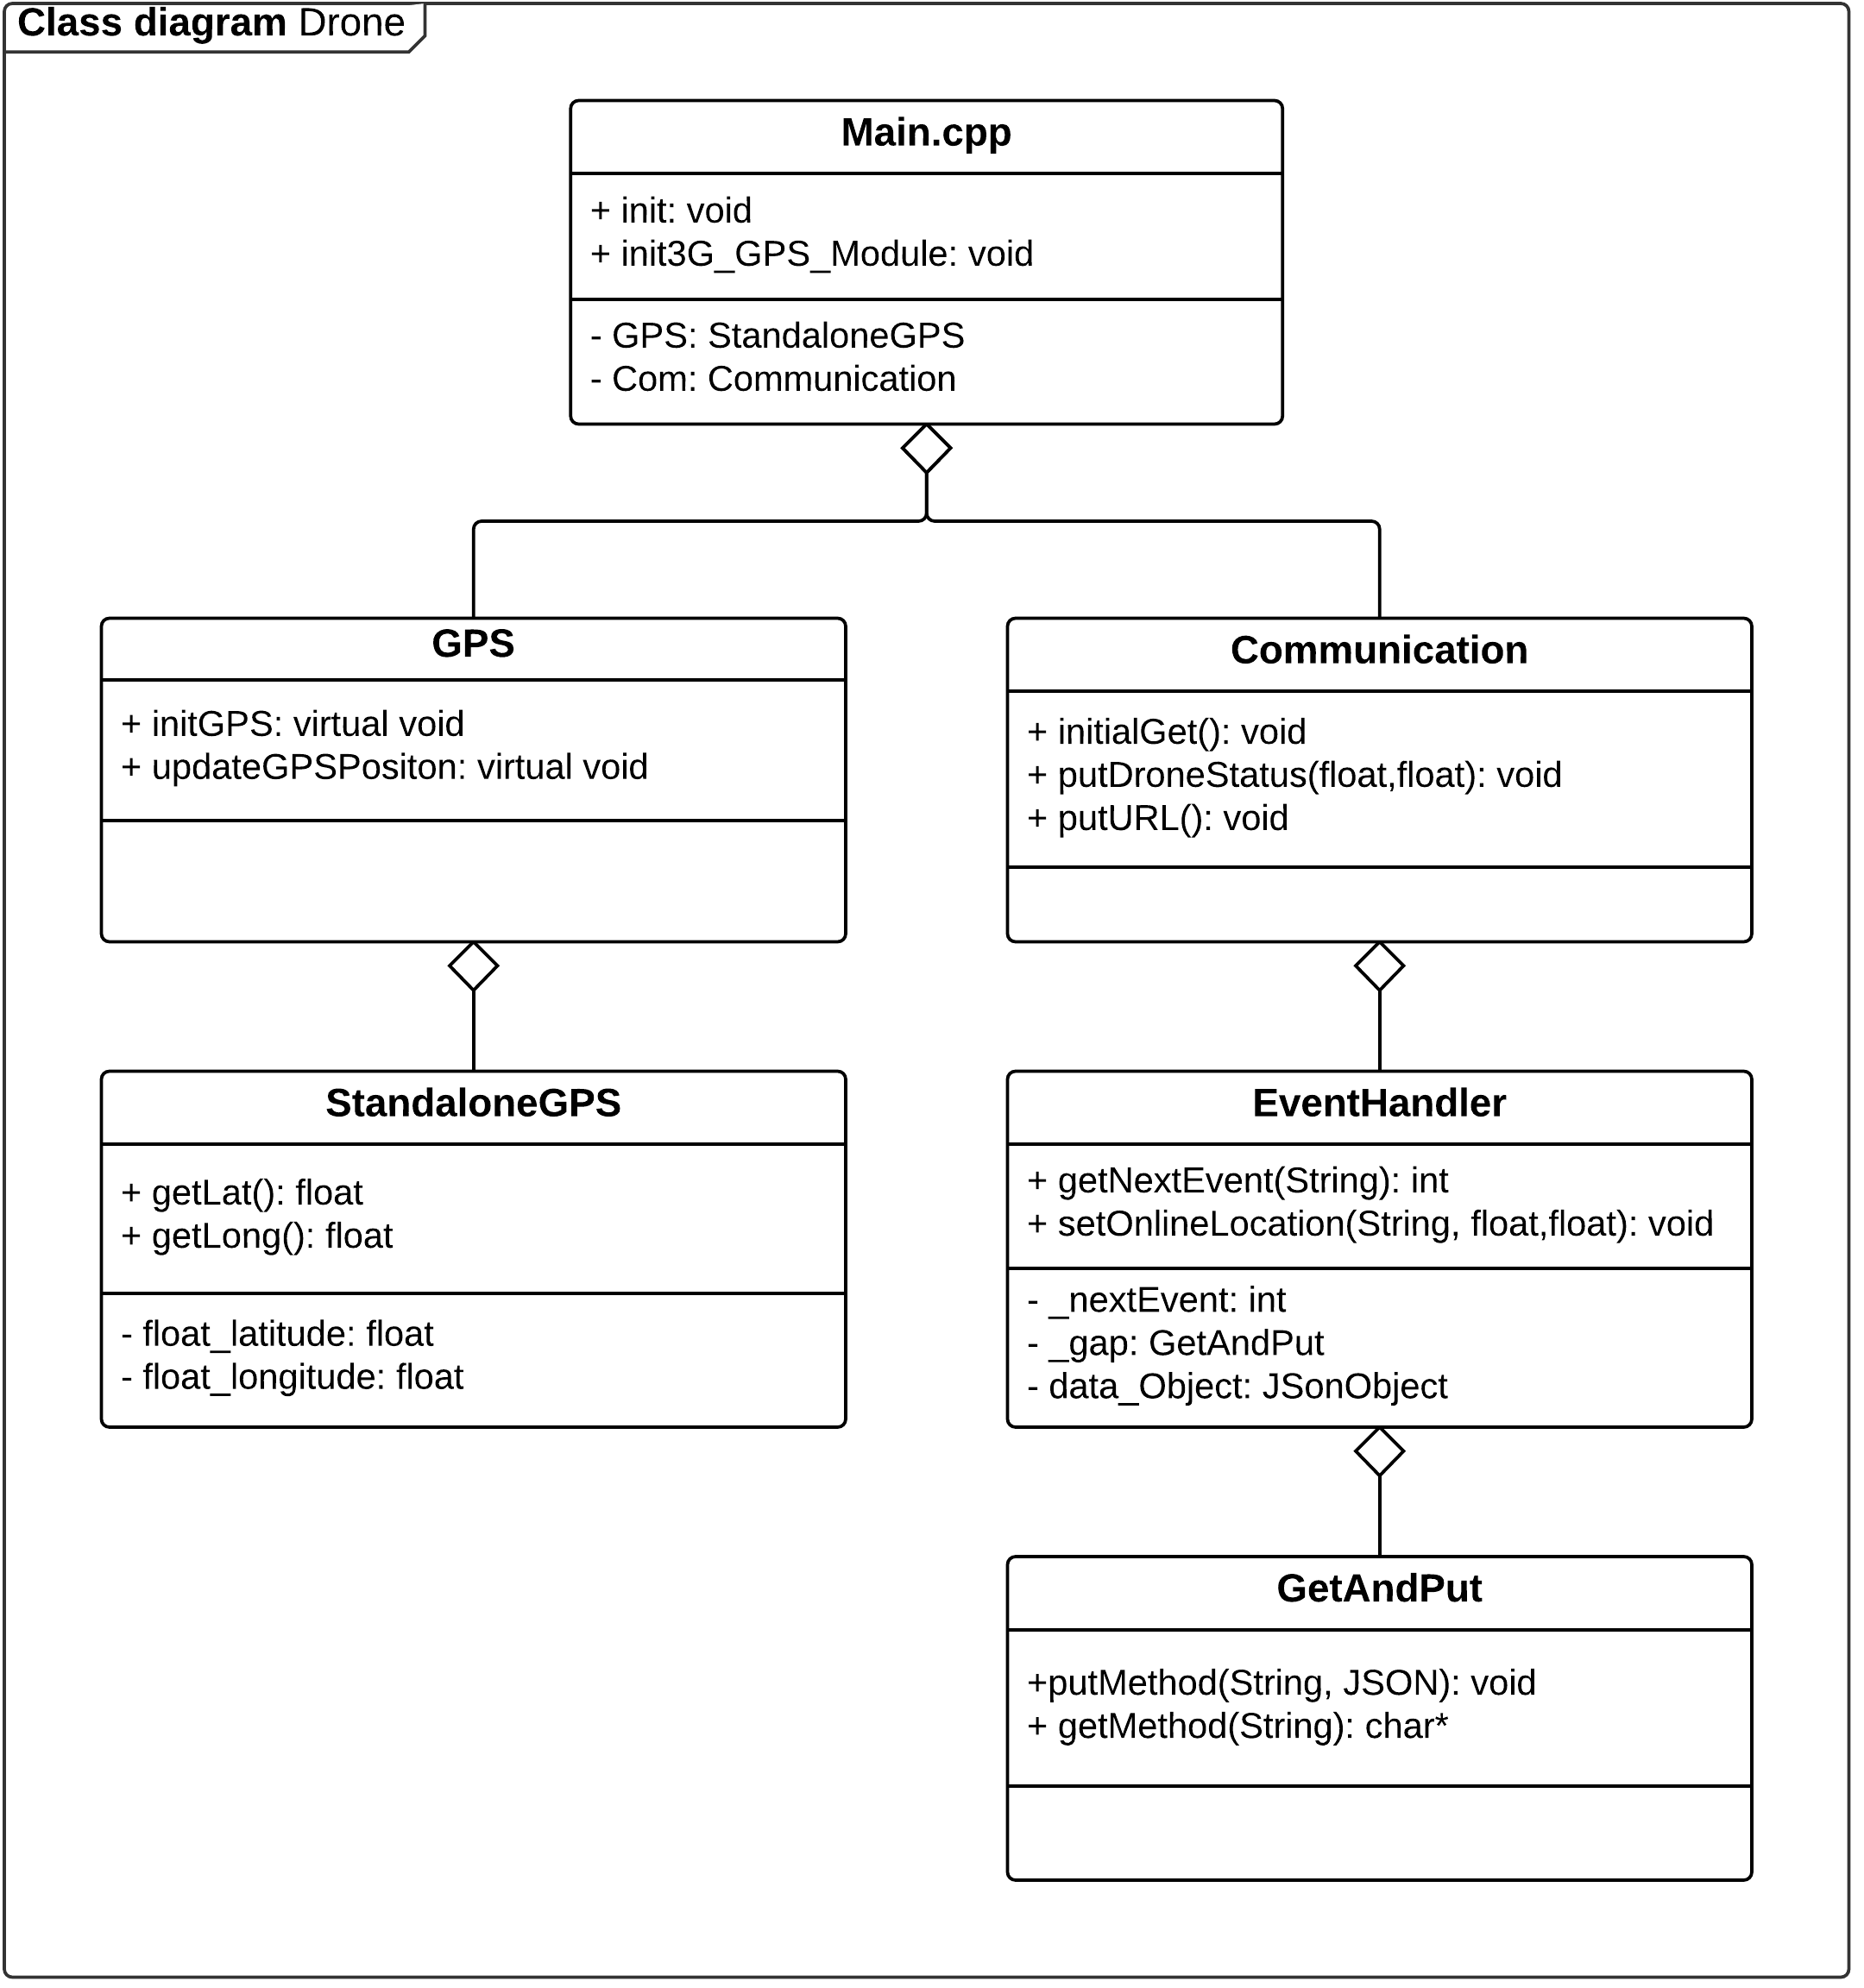
\includegraphics[width=1\textwidth]{Billeder/klasse_diagrammer/classdiagram_iteration1.png}
	\vspace{-0.5cm}
	\caption{Klassediagram drone}
	\label{fig:classDiagram_iteration1}
\end{figure}

\newpage

\textbf{Main.cpp} \\
Main.cpp filen bruges til at sætte arduino board korrekt op, bla. sættes baudrate på de forskellige serielle forbindelser. Desuden bruges Main.cpp til at kalde og eksekverer forskellige klasse, objekter og funktioner.

\textbf{GPS} \\
GPS klassen er implementeret som en abstract klasse. Init og updateGPSPosition er lavet som virtuelle metoder, hvilket betyder de skal implementeres i alle afledte klasser. GPS klassen er lavet fordi 3G/GPS modulet kunne bruges i 3 forskellige GPS modes. 

\textbf{StandaloneGPS}\\
Denne klasse er ansvarlig for al kommunikation med GPS'en når standalone mode er valgt. 

\textbf{GetAndPut} \\
GetAndPut klassen er den klasse der er tættest på hardwaren. Klassen indeholder http metoder der bruges til kommunikation mellem dronen og serveren. 

\textbf{Communication} \\
Communication klassen styrer alt der har med 3G kommunikation at gøre.

\textbf{EventHandler} \\
EventHandler klassen håndterer Events, og bruges som bindeled mellem communication- og GetAndPut klassen. EventHandleren sorterer eventID'et fra data der modtages og returnerer værdien af eventID til communication klassen. 


\newpage

\subsubsection*{Klassediagram webapplikation}
\vspace{-0.3cm}
Figur \ref{fig:classDiagram_webapplikation} viser klassediagrammet tilhørende webapplikation tilhørende iteration 1.

\vspace{-0.2cm}
\begin{figure}[H]
	\centering
	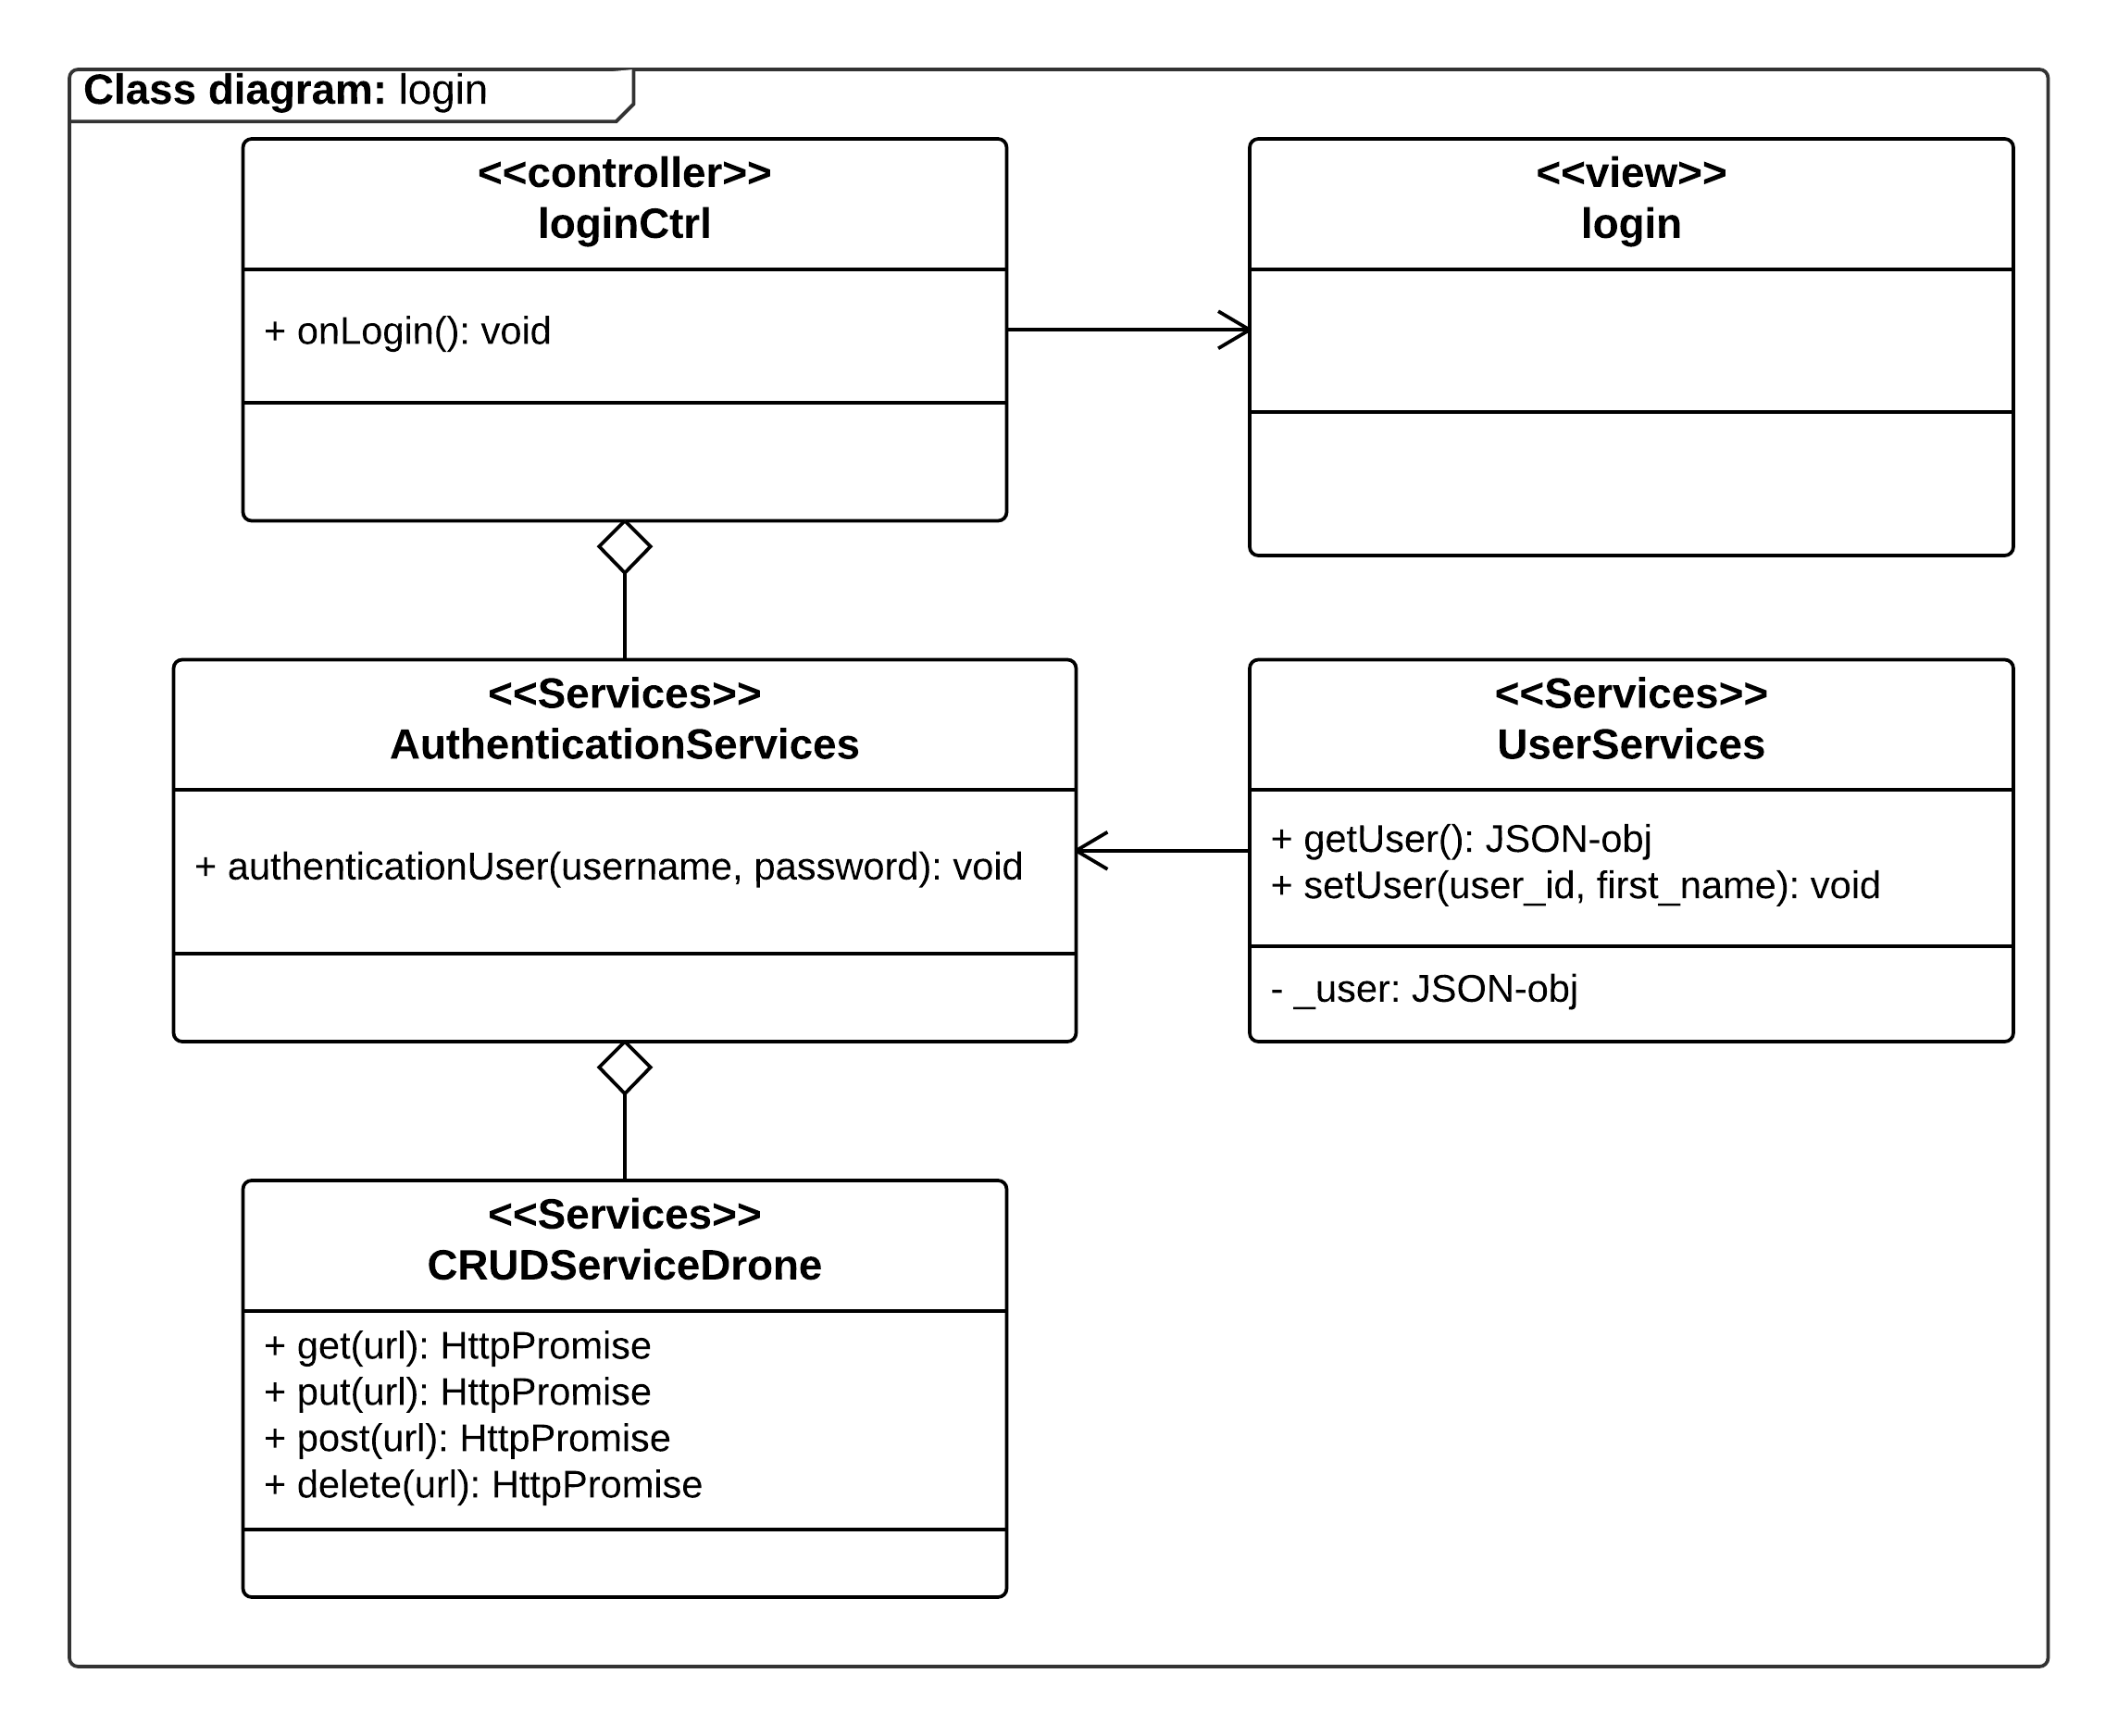
\includegraphics[width=1\textwidth]{Billeder/klasse_diagrammer/login_class_diagram.png}
	\vspace{-0.6cm}
	\caption{Klassediagram webapplikation}
	\label{fig:classDiagram_webapplikation}
\end{figure}

\vspace{-0.2cm}

\textbf{login} \\
Denne klasse er view'et tilhørende iteration 1. Sammen med loginCtrl skaber Login klassen det view som bruger ser i sin browser.

\textbf{loginCtrl} \\
LoginCtrl er en controller klasse som er forbundet med view klassen via two-way databinding. Klassen uddelegere også opgaver til dens services.

\textbf{AuthenticationServices} \\
AuthenticationServices klassen er ansvarlig for at afgøre om bruger er authenticated eller ej. Hvis bruger er authenticated bliver han/hun redirected til webapplikations home-page. Klassen gør brug af UserServices klassen til at gemme information om den bruger der er logget ind på webapplikationen.

\textbf{UserServices}\\
UserServices bruges til at gemme information om hvilken bruger der er logget ind på webapplikationen.

\textbf{CRUDServicesDrone} \\
Denne klasse bruges som bindeled imellem server og webapplikation, og indeholder logik til serveren. CRUDServicesDrone bruges når der sendes Get, Put og Post til serveren.


\subsubsection*{State machine diagram}
\vspace{-0.1cm}
I state machine diagrammet på figur \ref{fig:Statemachine_iteration1}, vises de forskellige states der eksisterer i iteration 1 og hvordan flowet imellem dem ser ud. Der eksisterer givet vis kun 1 state i iteration 1, men state machinen er medtaget fordi der bygges ovenpå den i de efterfølgende iterationer.
%kommentar
\begin{figure}[H]
	\centering
	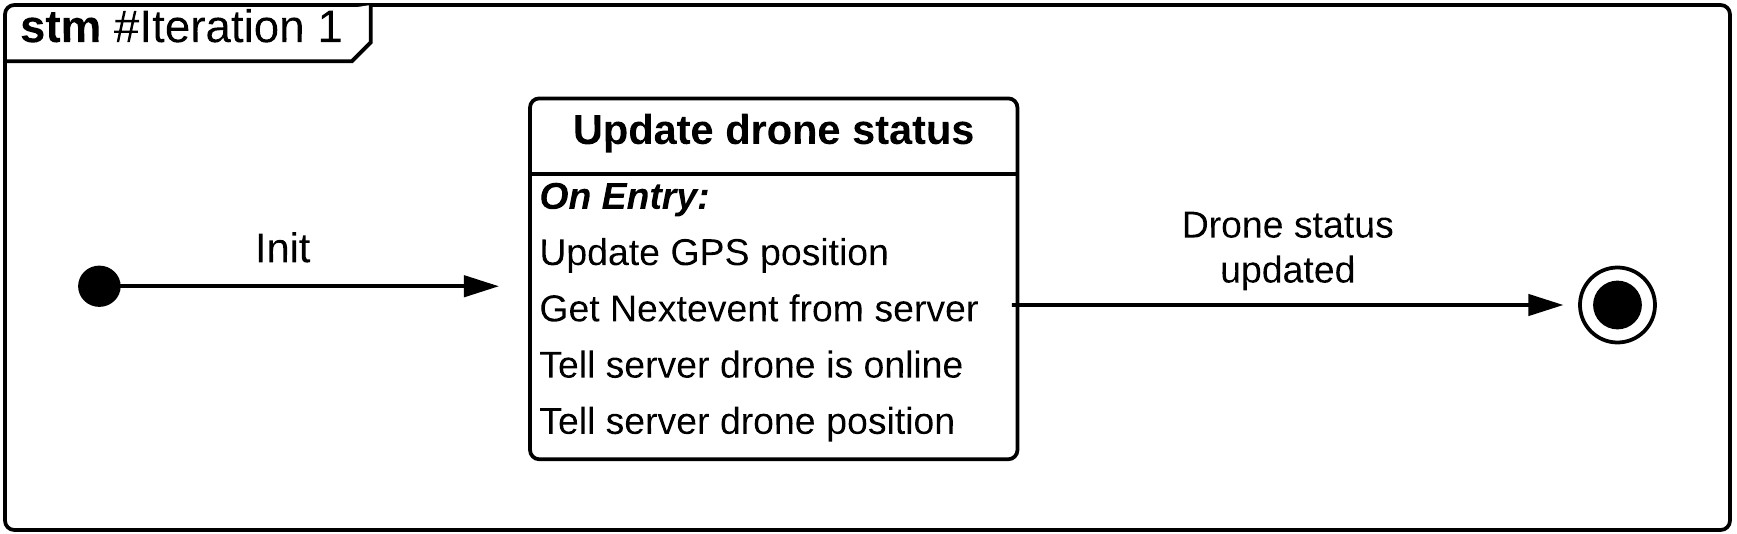
\includegraphics[width=1\textwidth]{Billeder/statemachine/State_iteration1.png}
	\vspace{-0.5cm}
	\caption{State machine}
	\label{fig:Statemachine_iteration1}
\end{figure}